\documentclass[12pt]{article}

\usepackage[T1]{fontenc}
\usepackage[utf8]{inputenc}
\usepackage[margin=1in]{geometry}
\usepackage{setspace}
\usepackage{booktabs}
\usepackage{amsmath}
\usepackage{graphicx}
\usepackage{hyperref}
\usepackage{xurl}
\usepackage{array}
\usepackage{lmodern}
\usepackage{microtype}
\usepackage{caption}

\onehalfspacing

\title{Kazakhstan and China in the Framework of Economic Diplomacy:\\
Trade Cooperation and Emerging Challenges, 2015--2024}
\author{}
\date{}

\hypersetup{
    colorlinks=true,
    linkcolor=black,
    citecolor=black,
    urlcolor=blue
}

\captionsetup{
    font=small,
    labelfont=bf
}

\begin{document}

\maketitle

\begin{abstract}
This paper examines the structural evolution of Kazakhstan--China trade relations between 2015 and 2024 through the lens of world-systems theory. Rather than treating the relationship primarily as a case of bilateral interdependence or direct dependence, it argues that the more important issue is the persistent core--periphery division embedded in the composition of trade. Across the period, Kazakhstan continued to export crude oil, metals, uranium, and other raw or minimally processed commodities to China, while importing a growing volume of higher-value manufactured goods. Using bilateral trade data from the World Bank WITS database, sectoral composition analysis, and formula-based tests (Trade Intensity Index, Revealed Comparative Advantage, Export Concentration Index, Trade Complementarity Index, and Terms of Trade), the paper finds consistently high trade intensity (TII above 4), persistent export concentration (HHI about 0.32--0.42), rising complementarity after 2020 (TCI peaking around 20.86 in 2022), and volatile but improving post-2020 terms of trade. These method and test results show that Kazakhstan's vulnerability lies less in the sheer amount of trade with China than in the developmental consequences of commodity specialization. The findings suggest that Kazakhstan is not best understood as simply dependent on China in a volume-based sense. Its longer-run risk is structural lock-in within a pattern of exchange that may constrain industrial upgrading, diversification, and movement into higher value-added sectors. The paper concludes that multivector diplomacy alone cannot resolve this problem without domestic industrial policy and export diversification capable of altering Kazakhstan's position in the bilateral value chain.
\end{abstract}

\noindent\textbf{Keywords:} Kazakhstan, China, world-systems theory, core--periphery, trade structure, economic diplomacy, multivector policy

\section{Introduction}

Kazakhstan's bilateral trade with China expanded sharply between 2015 and 2024. Trade values nearly tripled, China's role as an import supplier grew, and Chinese automotive, electronic, and industrial goods filled market space altered by the Russia--Ukraine war and the disruption of Eurasian trade routes (MERICS, 2022; Stronski and Sokolsky, 2024; Lim et al., 2025). These changes occurred within Kazakhstan's long-standing doctrine of multivectorism, which seeks balanced engagement with China, Russia, the European Union (EU), and other partners in order to preserve foreign-policy autonomy (Contessi, 2015; Clarke, 2015).

The question is not simply whether Kazakhstan trades more with China than it did a decade earlier. It plainly does. The more important question is what kind of trade relationship has developed. If Kazakhstan's exports to China remain concentrated in crude oil, metals, uranium, and other primary goods while imports from China consist mainly of machinery, vehicles, electronics, and consumer manufactures, then the developmental implications are different from those suggested by aggregate trade growth alone. A rising trade relationship can deepen connectivity while leaving the smaller economy in a structurally peripheral position.

This paper argues that the main risk in Kazakhstan's economic relationship with China is not simple bilateral dependence, but a persistent core--periphery trade structure in which Kazakhstan exports raw materials and imports higher value-added manufactures, thereby constraining long-run diversification and industrial upgrading. The paper therefore focuses on the composition of trade rather than trade volume alone, and evaluates this structure using sectoral trade evidence, Revealed Comparative Advantage, export concentration, trade complementarity, and terms-of-trade logic.

The paper proceeds in ten sections. After reviewing the relevant literature, it develops a world-systems theoretical framework, explains the data and methodology, presents the main results, analyzes Kazakhstan's external trade structure, examines the commodity--manufacture divide in Sino-Kazakh trade, discusses developmental risk, considers practical strategies for small and middle powers, and concludes with policy implications.

\section{Literature Review}

Scholarship on Kazakhstan--China economic relations has developed around three broad themes: the Belt and Road Initiative (BRI), Kazakhstan's multivector foreign policy, and the political economy of Chinese economic activity in Central Asia. Kazakhstan occupies a central position in BRI scholarship because Xi Jinping announced the initiative in Astana in 2013 and because Kazakhstan's geography is essential to overland Eurasian corridors. Studies of the BRI in Kazakhstan have emphasized infrastructure connectivity, transit potential, energy cooperation, investment, and the state's attempt to convert geographic location into diplomatic and commercial leverage (Kassenova, 2017; Bitabarova, 2019; World Bank Group, 2020; Pepe, 2021).

The most recent comprehensive discussion of China--Kazakhstan economic ties by Lim, Tjia, and Murashkin (2025) argues that Kazakhstan has avoided structural dependency and that BRI-era trade has become more balanced over time. Other work is more cautious. The Mercator Institute for China Studies (MERICS) (2022) argues that Russia's weakening position after the invasion of Ukraine has increased China's economic importance for Kazakhstan. Castellano and Castillo (2024) show that Chinese state capital can contribute to downstream resource development, but that outcomes vary by project and sector. Studies of Central Asian foreign policy also emphasize that multivectorism can preserve diplomatic maneuverability without necessarily transforming underlying economic structures (Contessi, 2015; Stronski and Sokolsky, 2024).

Existing scholarship on Kazakhstan--China economic relations has documented the growth of trade, transit connectivity, and BRI-related infrastructure. However, much of this literature emphasizes connectivity, investment scale, or short-run bilateral balance rather than the developmental implications of trade composition. This paper shifts the focus from whether Kazakhstan is becoming dependent on China in a narrow bilateral sense to whether the structure of exchange increasingly resembles a core--periphery pattern in which Kazakhstan remains concentrated in commodity exports while China supplies higher value-added manufactured goods.

The paper also draws on small-state and middle-power strategy debates. Hedging theory explains how states avoid exclusive alignment with a single great power while maintaining multiple channels of cooperation (Goh, 2007; Kuik, 2008). Institutional balancing theory similarly shows how smaller states can use institutions, rules, and multilateral settings to improve bargaining conditions without direct military confrontation (He, 2008). These approaches are useful, but this paper treats them as incomplete unless connected to domestic development. For Kazakhstan, external balancing only matters economically if it improves the country's capacity to move into higher value-added production.

\section{Theoretical Framework}

This paper uses world-systems theory as its primary analytical framework. In Wallerstein's formulation, the world economy is organized hierarchically between core, semi-peripheral, and peripheral zones. Core economies tend to specialize in capital-intensive and technologically advanced production and export higher value-added manufactured goods, while peripheral economies are more likely to specialize in raw materials, extractive sectors, and lower value-added activities. The central issue is therefore not simply who trades more with whom, but how the structure of exchange distributes value creation, industrial upgrading, and long-run developmental opportunities.

Applied to Kazakhstan--China trade, this framework suggests that the key asymmetry is not adequately captured by bilateral trade balance alone. Kazakhstan is not best described as fully dependent on China in a narrow trade-volume sense, since China is important but not exclusive in Kazakhstan's overall trade portfolio, and Kazakhstan is likewise not among China's most important trade partners globally. Yet the composition of bilateral exchange maps closely onto a core--periphery pattern: Kazakhstan exports predominantly raw or lightly processed commodities, while China exports machinery, vehicles, electronics, and other manufactured goods with higher value-added content.

This structure matters because persistent specialization in primary exports can generate long-run developmental constraints. Commodity concentration exposes peripheral economies to price volatility, weaker technological spillovers, and limited backward and forward linkages compared with manufacturing-based development. In this sense, the main issue is not whether Kazakhstan has already become dependent on China in aggregate trade-share terms, but whether its role in bilateral trade is reinforcing a peripheral position that makes diversification more difficult over time.

The empirical analysis therefore evaluates the Kazakhstan--China relationship through several structural indicators. Revealed Comparative Advantage identifies whether Kazakhstan's sectoral strengths remain concentrated in extractive and low-processed goods. The Export Concentration Index captures how narrowly exports are distributed across product categories. The Trade Complementarity Index measures how closely Kazakhstan's export profile matches China's import demand, helping show whether complementarity is concentrated in raw materials rather than diversified industrial goods. Terms-of-trade logic is then used to interpret the developmental implications of exchanging commodities for manufactures over time.

This framework leads to a narrower and clearer argument: Kazakhstan's principal risk in its economic relationship with China is not simple bilateral dependence, but structural specialization in a commodity--manufacture exchange pattern that may undermine long-run industrial upgrading.

\section{Data and Methodology}

\subsection{Data Sources}

Bilateral trade and investment data are drawn primarily from the World Bank's World Integrated Trade Solution (WITS) database for Kazakhstan--China flows from 2015 to 2024. Product-level data are organized using Harmonized System (HS) categories and grouped into major sectors including energy, metals and minerals, chemicals, agriculture, machinery, vehicles, electronics, and other manufactures. For index construction, the paper uses (i) Kazakhstan--China bilateral and sectoral trade from the project panel, (ii) China imports from world and world imports aggregates from WITS raw comma-separated values (CSV) pulls, and (iii) Kazakhstan unit-value indicators from World Development Indicators (WDI) for export and import unit value indices. Supplementary information on Chinese investment and corridor policy is taken from Kazakhstan's National Bank, the Asian Development Bank, the World Bank, and policy documents cited in the literature.

\subsection{Data Processing and Reproducibility}

All quantitative results, indices, tables, and figures in this paper were compiled by the author using Stata do-files in the project workflow. The analysis pipeline imports raw data from WITS and WDI, constructs harmonized sectoral panels, and computes TII, RCA, HHI, TCI, and ToT directly from those source datasets. No quantitative table or figure was copied from external publications; all reported values are author-generated from the cited primary data sources.

\subsection{Trade Intensity Index}

The Trade Intensity Index (TII) is used here only as a descriptive indicator of bilateral salience, not as the paper's main measure of vulnerability. The core argument rests on sectoral composition and structural trade position rather than partner salience alone. Following Brown (1949), the index is:

\begin{equation}
TII_{ij} = \frac{x_{ij}/X_i}{m_j/M_w}
\end{equation}

\noindent where $x_{ij}$ is Kazakhstan's exports to China, $X_i$ is Kazakhstan's total world exports, $m_j$ is China's total world imports, and $M_w$ is total world merchandise imports. A value above 1 indicates that bilateral trade is more concentrated than global market shares would predict.

\subsection{Revealed Comparative Advantage}

To evaluate whether Kazakhstan's export structure has diversified beyond commodities, the paper uses the Balassa (1965) Revealed Comparative Advantage (RCA) index:

\begin{equation}
RCA_{ik} = \frac{x_{ik}/X_i}{x_{wk}/X_w}
\end{equation}

\noindent where $x_{ik}$ is Kazakhstan's exports of product $k$, $X_i$ is Kazakhstan's total exports, $x_{wk}$ is world exports of product $k$, and $X_w$ is total world exports. RCA values above 1 indicate revealed comparative advantage. The analysis focuses on whether Kazakhstan's strongest export categories to China remain concentrated in energy, metals, minerals, and other resource-based sectors.

\subsection{Trade Asymmetry Index}

The Trade Asymmetry Index (TAI) is retained only as a supplementary descriptive measure of short-run divergence between export and import growth. It is not treated as the main indicator of structural vulnerability in this paper, because temporary shifts in annual trade balance can be driven by shocks such as the pandemic, commodity price swings, and the Russia--Ukraine war. The revised argument instead rests on the persistent composition of trade, export concentration, and the commodity--manufacture divide.

\subsection{Core--Periphery Structure: World-Systems Indicators}

World-systems theory predicts that the Kazakhstan--China trade relationship reproduces a core--periphery structure in which China exports higher value-added manufactured goods while Kazakhstan exports raw materials and low-processed commodities. To operationalize this structural claim and distinguish it from a simple trade-volume or trade-deficit narrative, the paper employs three additional quantitative measures alongside RCA: the Export Concentration Index (HHI), the Trade Complementarity Index (TCI), and terms-of-trade analysis.

\paragraph{Export Concentration Index (HHI).}
The Herfindahl--Hirschman Index measures the degree to which Kazakhstan's export basket to China is concentrated in a narrow set of sectors:
\begin{equation}
\text{HHI}_t = \sum_{p=1}^{n} s_{p,t}^2
\end{equation}
\noindent where $s_{p,t}$ is the share of product $p$ in Kazakhstan's exports to China in year $t$. Higher values indicate stronger concentration and therefore greater reliance on a limited number of export categories.

\paragraph{Trade Complementarity Index (TCI).}
The Trade Complementarity Index captures the degree to which Kazakhstan's export structure matches China's import demand:
\begin{equation}
\text{TCI}_{ij,t} = 100 \times \left(1 - \frac{\sum_{p}\left|m_{p,j,t} - x_{p,i,t}\right|}{2}\right)
\end{equation}
\noindent where $m_{p,j,t}$ is the share of product $p$ in country $j$'s total imports in year $t$, and $x_{p,i,t}$ is the share of product $p$ in country $i$'s total exports in year $t$. In this paper, $i$ denotes Kazakhstan and $j$ denotes China. High complementarity does not by itself indicate balanced development; in this case, it may simply show that Kazakhstan fits efficiently into China's demand for raw materials.

\paragraph{Terms of Trade (ToT).}
Terms of trade are used here to capture the developmental implications of commodity--manufacture exchange:
\begin{equation}
\text{ToT}_t = \frac{P_{x,t}}{P_{m,t}} \times 100
\end{equation}
\noindent where $P_{x,t}$ is Kazakhstan's export price index and $P_{m,t}$ is its import price index. A deterioration in terms of trade implies that Kazakhstan must export more raw materials to purchase the same quantity of imported manufactures.

\subsection{Qualitative Component}

The qualitative component reviews bilateral agreements, corridor projects, localization roadmaps, and policy statements related to China--Kazakhstan economic cooperation. These documents are used to assess whether official policy instruments have altered the structure of trade or primarily expanded connectivity and transaction volume. Across these policy instruments, the main pattern is clear: diplomatic agreements, logistics corridors, and localization roadmaps have expanded connectivity and commercial exchange, but they have not produced a clear shift in Kazakhstan's structural position within bilateral trade. The measurable pattern remains one of commodity exports from Kazakhstan and manufactured imports from China. The qualitative evidence therefore complements the quantitative analysis by showing that policy ambition has exceeded structural transformation.

Because the revised argument centers on structural trade composition rather than short-run dependence dynamics, regression-based tests of balance shifts are treated as secondary and omitted from the main analysis.

\section{Results}

\subsection{Trade Structure: China's Growing Role Without Full Bilateral Dependence}

The results show that China's role in Kazakhstan's trade increased over the period, but not in a way that justifies the strongest version of a bilateral dependence claim. The more consistent pattern is structural: Kazakhstan's exports to China remain concentrated in raw materials and low-processed goods, while imports from China are dominated by higher value-added manufactures. This asymmetry is visible across sectoral composition, RCA patterns, export concentration, and the qualitative record of failed diversification efforts.

China's share of Kazakhstan's external trade increased between 2015 and 2024, especially on the import side. However, this increase should not be overstated as evidence of full bilateral interdependence, since Kazakhstan continues to trade substantially with the European Union and Russia, while Kazakhstan remains a relatively limited partner from China's global perspective. The significance of China's growing role lies less in exclusivity than in the fact that its rise has occurred alongside the persistence of a commodity--manufacture division of labor.

\begin{table}[h]
\centering
\caption{Kazakhstan--China Bilateral Trade, 2015--2024. Source: author's calculations from WITS data.}
\label{tab:bilateral-trade}
\begin{tabular}{rrrrr}
\toprule
Year & Exports to China & Imports from China & Balance & Total Trade \\
 & \multicolumn{4}{c}{US\$ billions} \\
\midrule
2015 & 10.96 & 10.18 & 0.78 & 21.14 \\
2016 & 8.43 & 7.33 & 1.10 & 15.75 \\
2017 & 11.60 & 9.39 & 2.21 & 20.99 \\
2018 & 12.61 & 10.77 & 1.85 & 23.38 \\
2019 & 16.01 & 13.58 & 2.43 & 29.58 \\
2020 & 13.67 & 3.91 & 9.76 & 17.58 \\
2021 & 13.70 & 4.85 & 8.86 & 18.55 \\
2022 & 20.92 & 7.15 & 13.77 & 28.07 \\
2023 & 29.52 & 33.54 & -4.03 & 63.06 \\
2024 & 29.79 & 30.31 & -0.51 & 60.10 \\
\bottomrule
\end{tabular}
\end{table}

As shown in Table~\ref{tab:bilateral-trade}, the 2023 deficit is best interpreted as a warning sign rather than the core argument of the paper. It matters because it coincides with the persistence of commodity specialization, not because deficit alone proves dependence. Even if the bilateral balance shifts again in future years, the deeper developmental concern would remain the same so long as Kazakhstan continues to export mostly raw materials and import mostly higher value-added manufactures.

\begin{figure}[htbp]
\centering
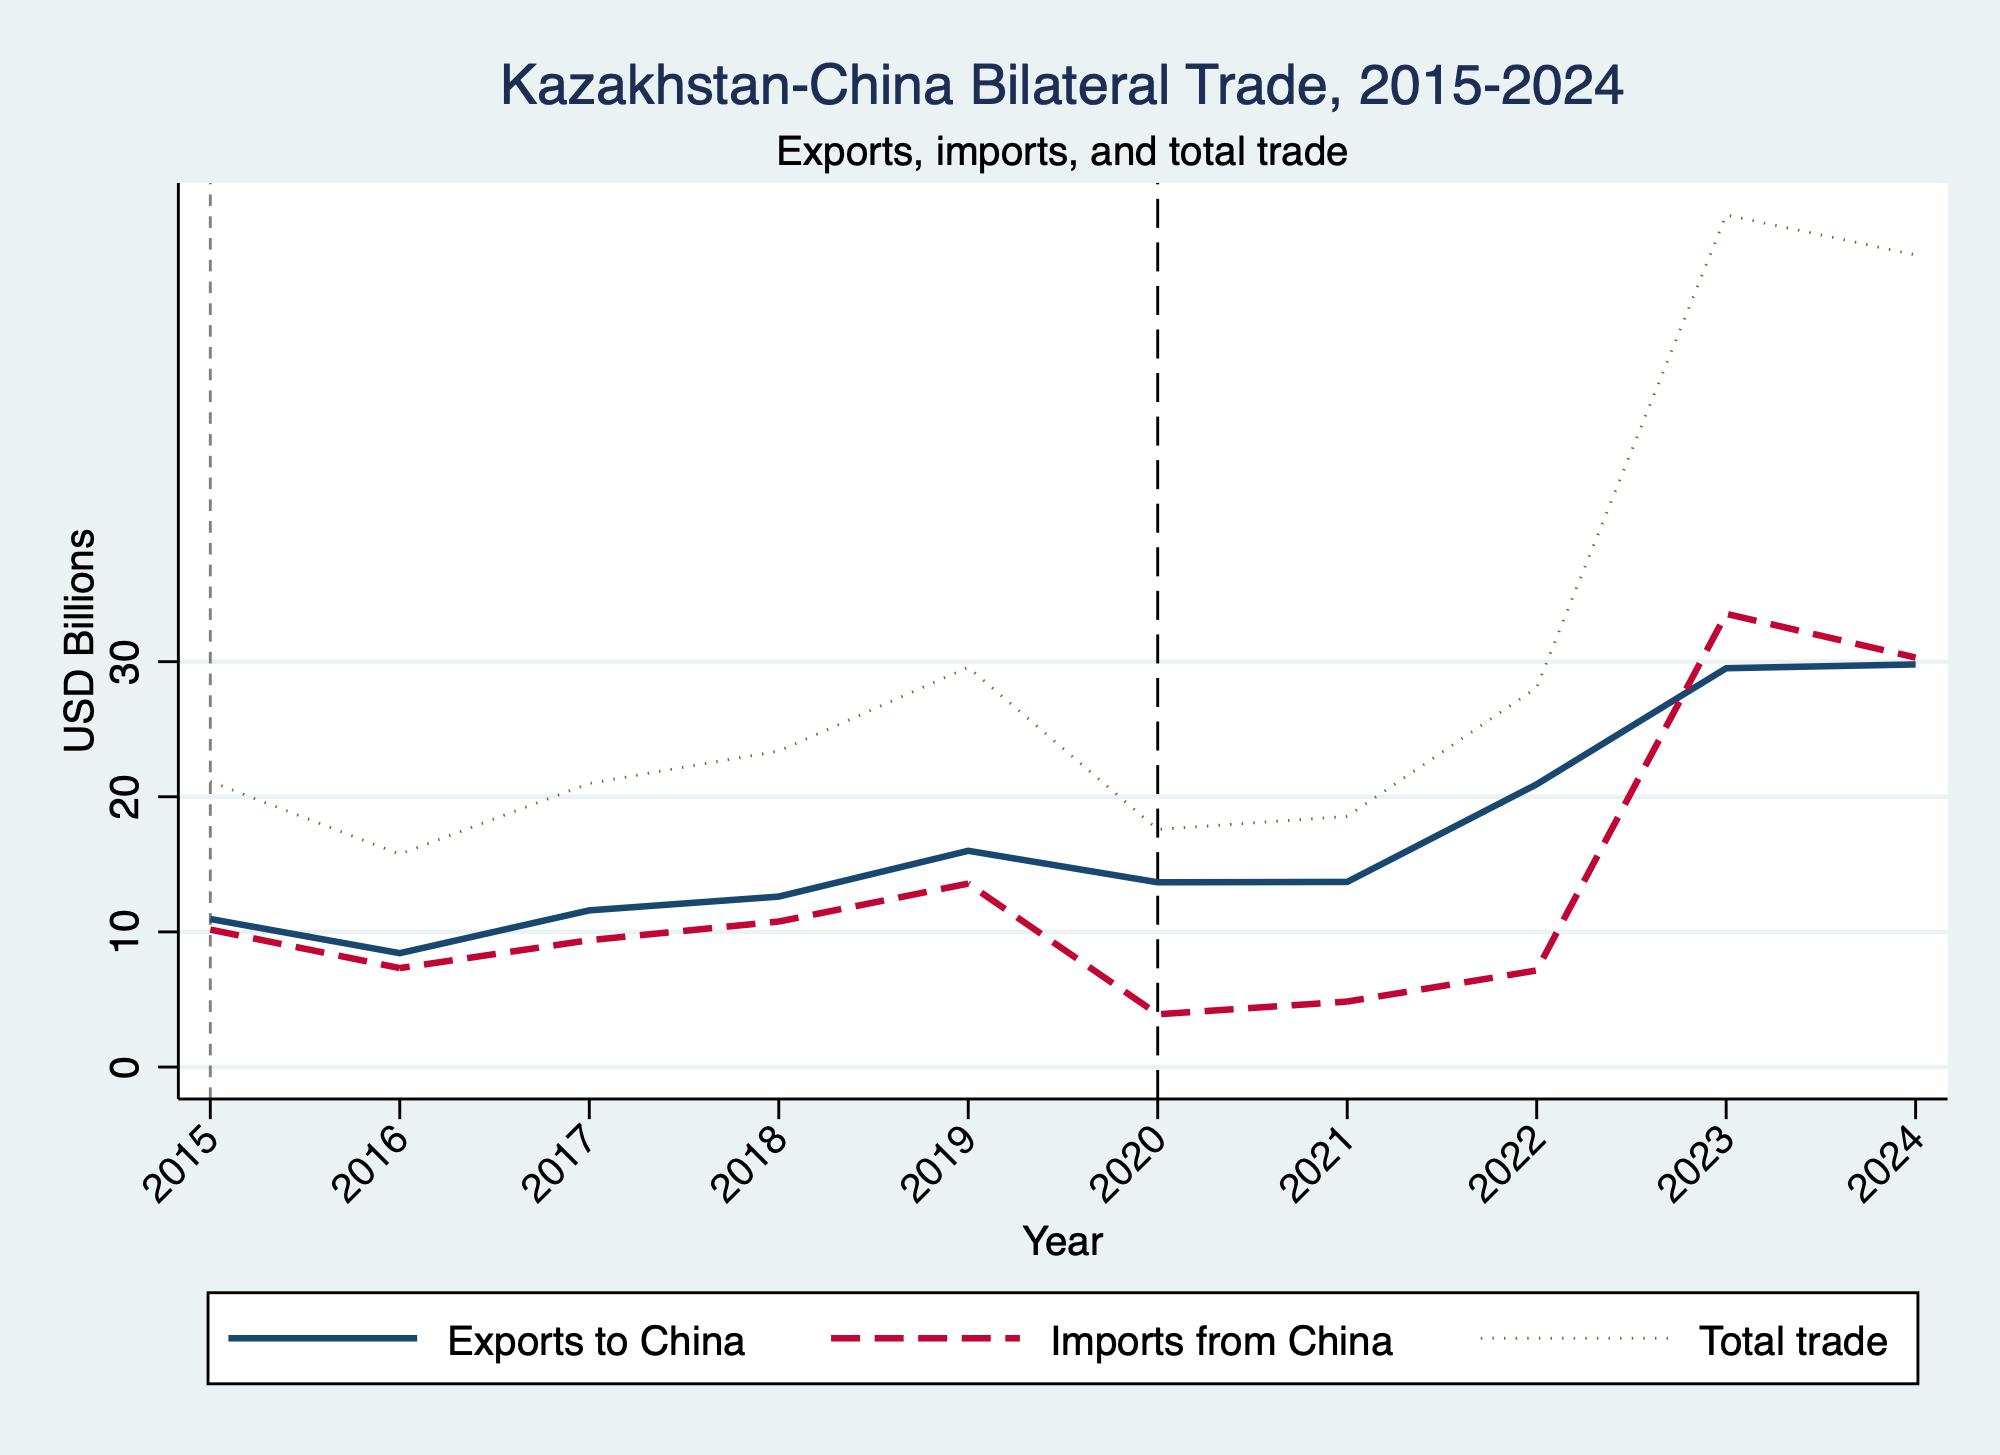
\includegraphics[width=0.95\textwidth]{../figures/fig12_trade_flows.png}
\caption{Kazakhstan--China bilateral trade flows, 2015--2024. Source: author's calculations from WITS data.}
\label{fig:trade-flows}
\end{figure}

\subsection{Formula-Based Index Results}

As shown in Figure~\ref{fig:trade-flows}, trade values expand sharply over the sample period. Table~\ref{tab:formula-indices} reports the annual values for the paper's formula-based indicators. TII remains above 4 in all years (4.17--5.71), indicating that Kazakhstan's export orientation toward China is stronger than China's weight in world imports would predict. Export concentration remains high throughout the period (HHI 0.32--0.42), consistent with a narrow commodity basket. TCI rises from roughly 13--15 in 2015--2019 to around 19--21 in 2020--2022 before easing in 2023--2024, indicating changing but still structurally limited complementarity. Terms of trade (ToT), computed as export unit value index over import unit value index, deteriorate in 2016 and 2020, improve strongly in 2021--2022, and moderate afterward.

\begin{table}[h]
\centering
\caption{Formula-Based Indices, 2015--2024. Source: author's calculations from WITS and WDI data.}
\label{tab:formula-indices}
\begin{tabular}{rrrrr}
\toprule
Year & TII & HHI (exports) & TCI & ToT \\
\midrule
2015 & 5.55 & 0.320 & 13.46 & 100.00 \\
2016 & 5.71 & 0.355 & 13.43 & 89.22 \\
2017 & 5.56 & 0.422 & 13.30 & 101.83 \\
2018 & 5.16 & 0.392 & 13.83 & 114.95 \\
2019 & 5.50 & 0.401 & 14.86 & 106.46 \\
2020 & 5.04 & 0.343 & 19.33 & 85.89 \\
2021 & 4.17 & 0.386 & 19.85 & 120.81 \\
2022 & 5.01 & 0.392 & 20.86 & 144.25 \\
2023 & 5.51 & 0.353 & 18.80 & 124.49 \\
2024 & 5.40 & 0.373 & 18.92 & 119.43 \\
\bottomrule
\end{tabular}
\end{table}

\subsection{Revealed Comparative Advantage: Persistent Commodity Specialization}

The RCA evidence indicates that Kazakhstan's comparative strengths remain concentrated in a narrow set of sectors under the paper's constructed world-baseline measure. Average RCA is highest in metals and minerals (2.96) and chemicals (2.49), while machinery and electrical goods (0.26), plastics and rubber (0.15), wood and paper (0.15), and stone and ceramics (0.01) remain well below 1. This pattern is consistent with limited movement into technologically complex exports to China.

The result is important because it qualifies optimistic interpretations of trade growth. Higher trade volume does not necessarily mean higher developmental capability. If Kazakhstan sells more of the same commodity categories while importing more advanced manufactured products, then integration may deepen without changing the country's position in the bilateral value chain. These RCA patterns indicate that Kazakhstan has not diversified into competitive higher value-added exports to China. Instead, comparative strength remains concentrated in extractive and resource-based sectors, which is consistent with a peripheral trade position under world-systems theory.

\subsection{Export Concentration and Commodity Specialization}

The export concentration evidence reinforces the RCA findings. Kazakhstan's export basket to China remains heavily concentrated in a narrow range of primary products, especially hydrocarbons, metals, and related raw materials. Even when annual trade balances fluctuate, this concentration matters more for long-run development because it indicates that integration with China has not translated into broader industrial upgrading or a more diversified export profile.

High complementarity between Kazakhstan's exports and China's import demand is therefore ambiguous (Table~\ref{tab:formula-indices}). It can indicate that the two economies fit together commercially, but the content of that fit matters. In this case, complementarity largely reflects China's demand for resources and Kazakhstan's supply of raw materials rather than Kazakhstan's entry into complex manufacturing or technology-intensive exports.

\begin{figure}[htbp]
\centering
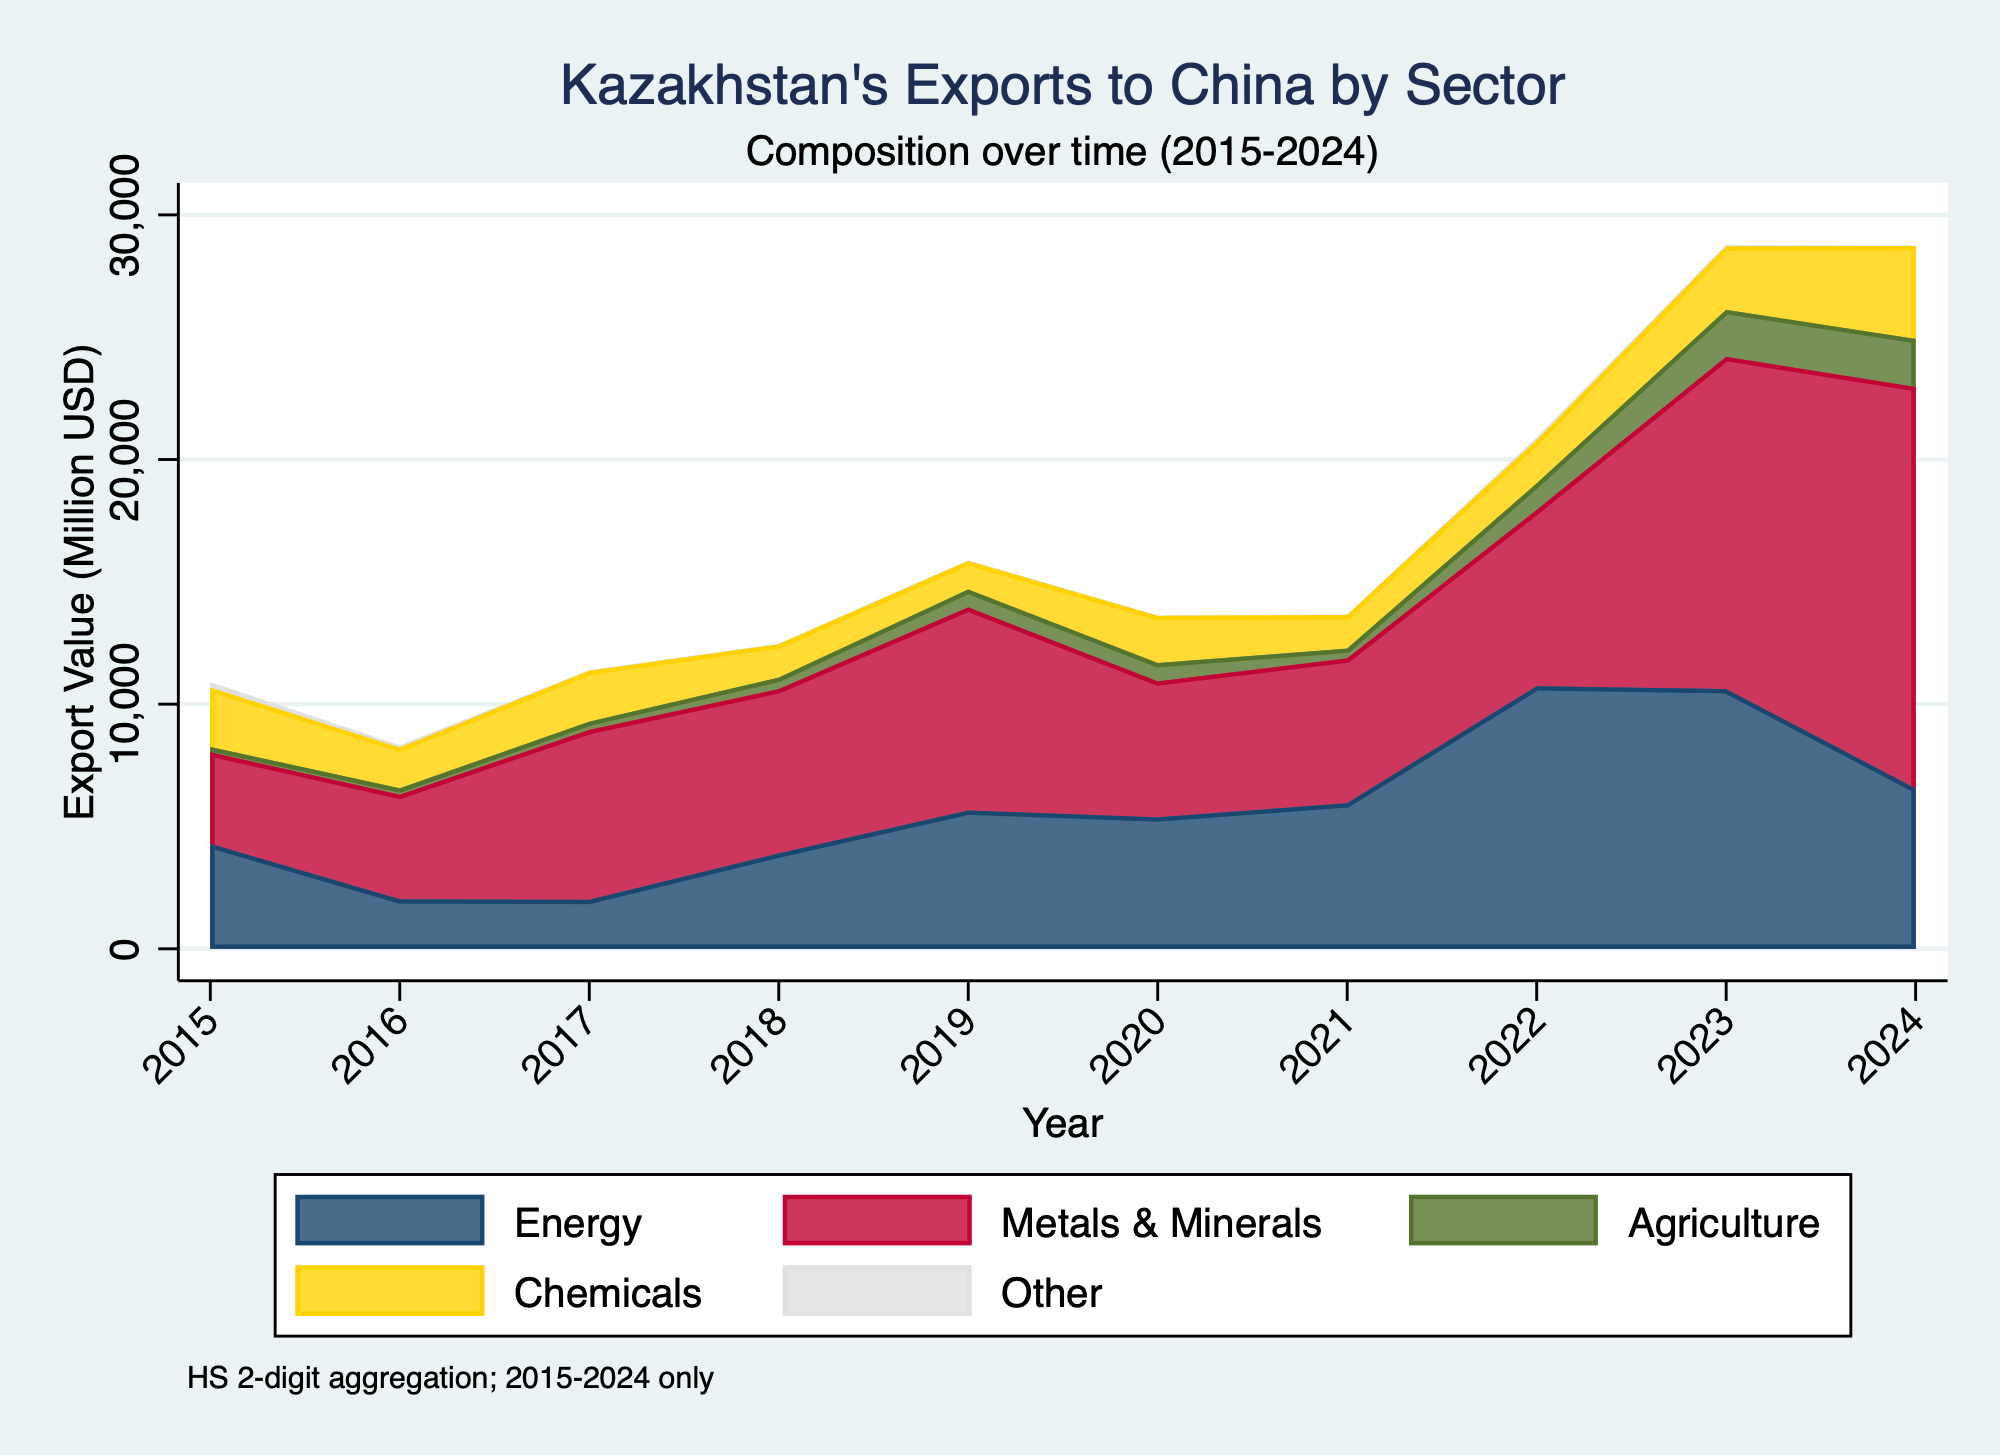
\includegraphics[width=0.95\textwidth]{../figures/fig1_export_composition.png}
\caption{Kazakhstan's exports to China by sector, 2015--2024. Source: author's calculations from WITS HS-level data.}
\label{fig:export-composition}
\end{figure}

\begin{figure}[htbp]
\centering
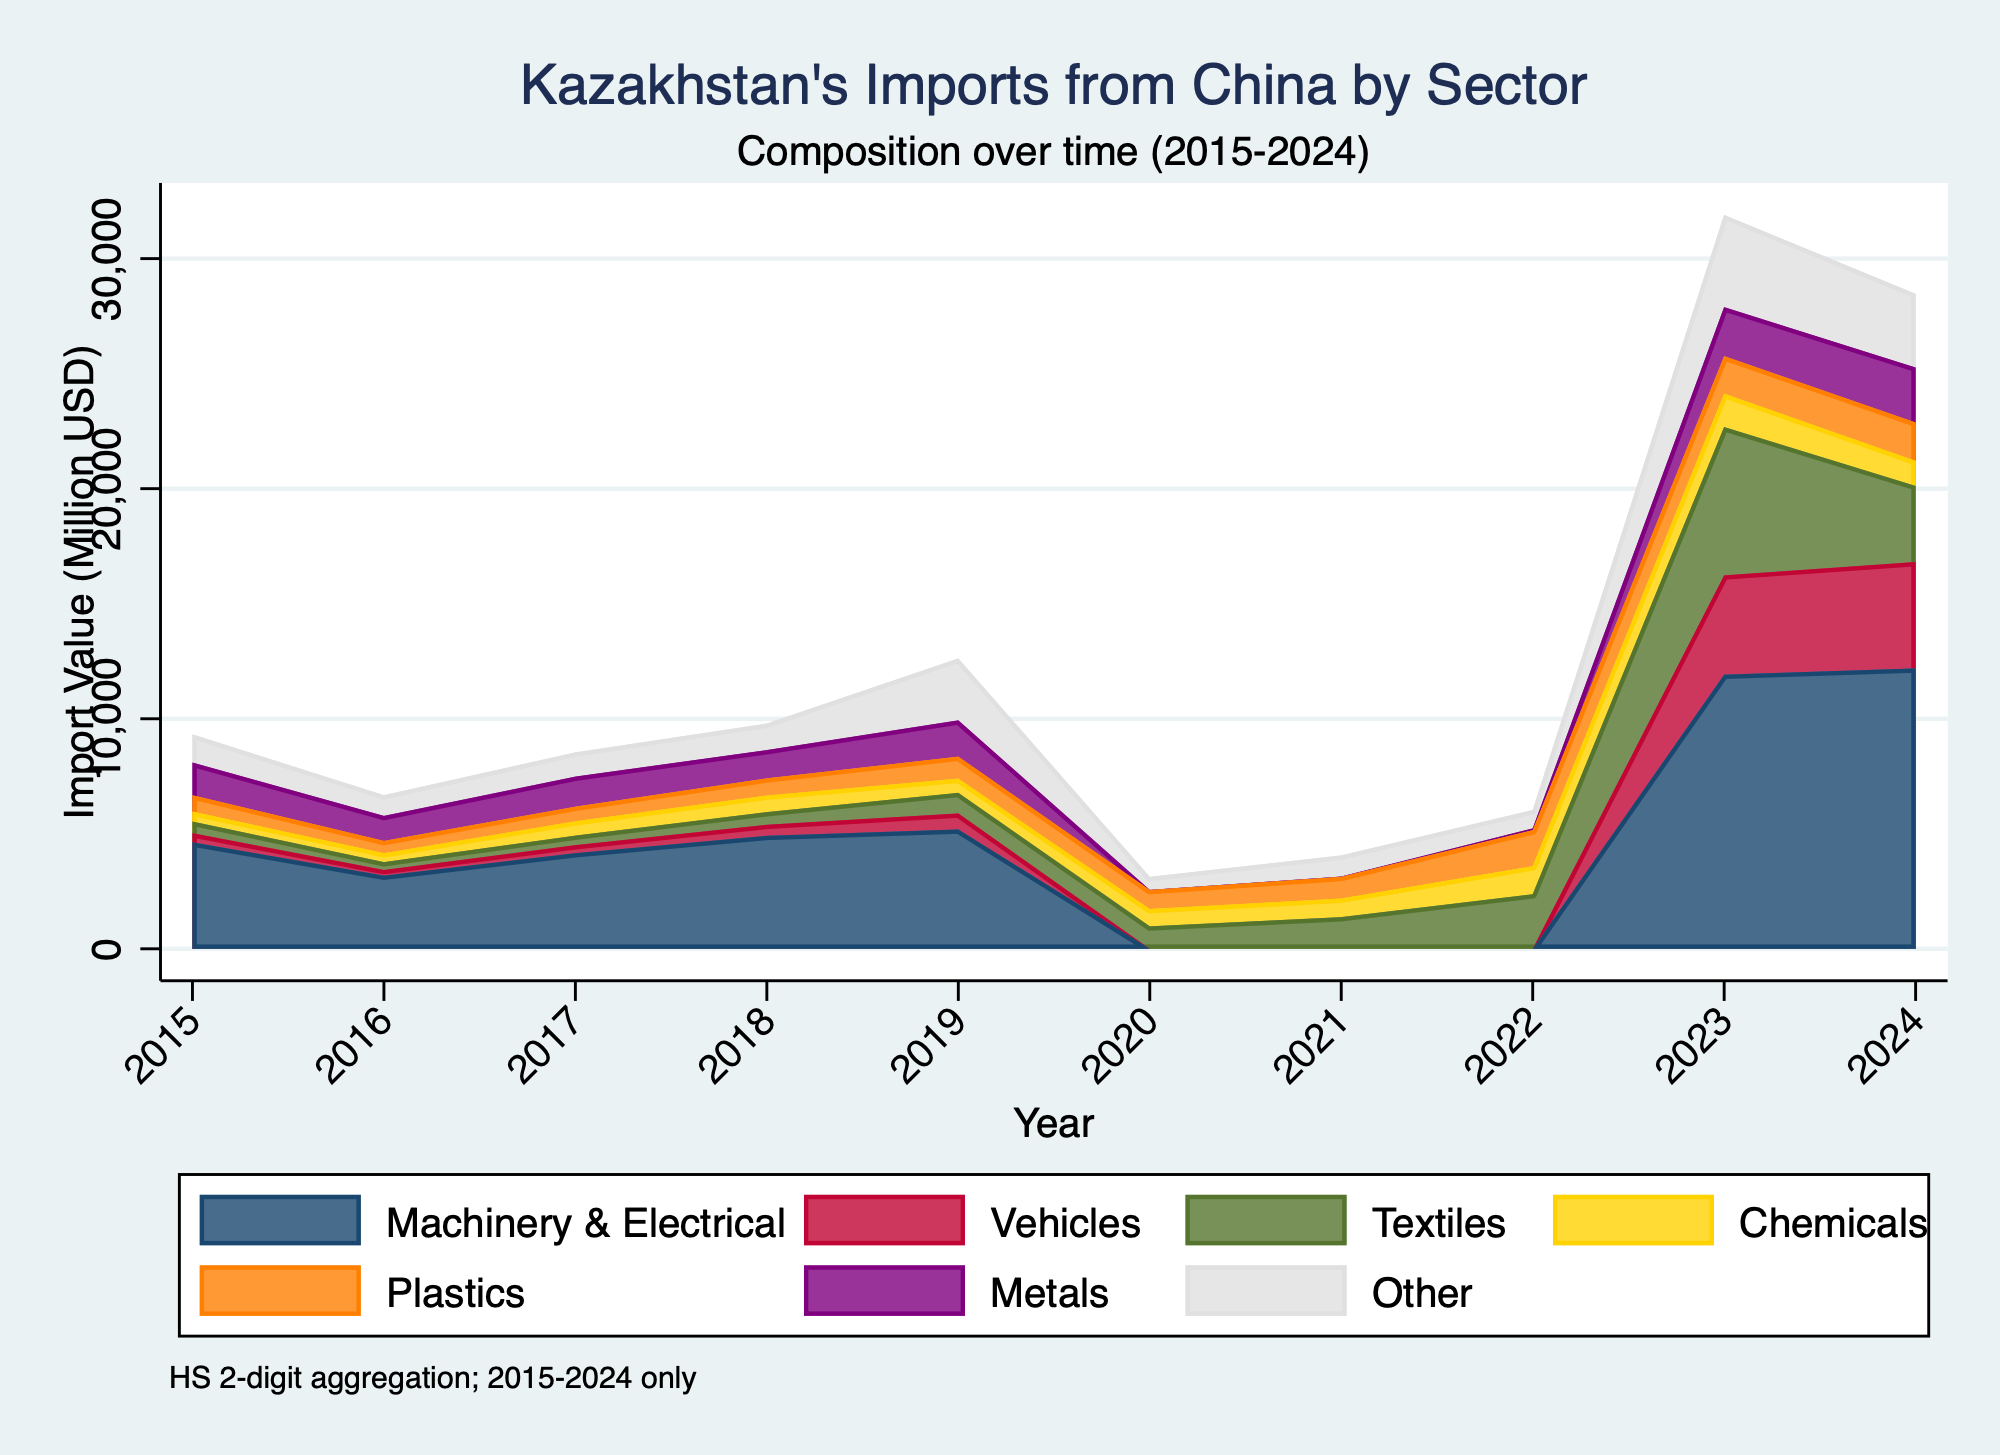
\includegraphics[width=0.95\textwidth]{../figures/fig2_import_composition.png}
\caption{Kazakhstan's imports from China by sector, 2015--2024. Source: author's calculations from WITS HS-level data.}
\label{fig:import-composition}
\end{figure}

\subsection{Policy Commitments Without Structural Diversification}

The qualitative evidence shows that bilateral agreements and corridor projects have been more effective at facilitating trade and transit than at changing Kazakhstan's structural role in that trade. Automotive assembly, transport infrastructure, and logistics cooperation have advanced in formal and operational terms, but these gains have not produced a visible shift toward higher value-added Kazakhstani exports. The result is a pattern of connectivity without commensurate structural transformation.

This does not mean that Kazakhstan lacks agency. Multivector diplomacy has helped maintain relations with multiple partners and has prevented China from becoming Kazakhstan's only significant economic relationship. But diplomatic diversification is not the same thing as productive diversification. A state may maintain several partners while still occupying a peripheral position in a specific and increasingly important bilateral trade structure.

\section{Kazakhstan's External Trade Structure, 2015--2024}

\subsection{The Multipolar Baseline and Its Erosion}

Kazakhstan's external trade in 2015 broadly reflected the logic of multivectorism, with the European Union, Russia, and China each playing important but differentiated roles. By 2024, China's share had risen, especially as an import supplier and transit partner (see Table~\ref{tab:bilateral-trade} and Figure~\ref{fig:trade-flows}). This shift is better interpreted as a change in Kazakhstan's structural trade position than as evidence of deep bilateral interdependence. China did not become Kazakhstan's only major economic partner, nor did Kazakhstan become one of China's central trade counterparts. What changed more clearly was the composition of exchange. As Chinese manufactured exports expanded and Kazakhstan's exports remained concentrated in crude oil, metals, uranium, and other primary goods, the bilateral relationship increasingly reflected a core--periphery pattern. The significance of this shift lies not simply in changing trade shares, but in the risk that continued commodity specialization will narrow Kazakhstan's long-run development options.

\subsection{The 2023 Trade Snapshot and Structural Risk}

Kazakhstan's 2023 trade accounts illustrate the structural asymmetry at issue in concrete terms. China was a leading destination for Kazakhstani exports and the largest source of imports, yet the more important fact is not the bilateral deficit alone. Running deficits with major import partners is less important here than the composition of exchange itself. The more significant pattern is that Kazakhstan continues to occupy the raw-material side of trade while importing higher value-added manufactured goods. This does not by itself prove bilateral dependence on China in a strict sense, but it does indicate a structural position associated with peripheral specialization and weaker prospects for industrial upgrading.

The post-2022 context sharpened this pattern. Russia's declining reliability as a trade and logistics partner increased the importance of China-linked routes, suppliers, and investment channels (MERICS, 2022; Stronski and Sokolsky, 2024). Yet this geopolitical opening did not produce a comparable increase in Kazakhstan's higher value-added exports. Instead, the main visible adjustment was the expansion of Chinese manufactured imports into Kazakhstan's domestic market.

\section{Structural Features of Sino-Kazakh Trade}

\subsection{Three Phases of Bilateral Trade Dynamics}

The bilateral relationship can be divided into three broad phases: pre-pandemic expansion, pandemic and post-pandemic disruption, and post-2022 realignment. Across these phases, annual trade values changed substantially, but the underlying pattern of exchange remained strikingly consistent. Kazakhstan exported commodities and imported manufactures, while policy initiatives failed to generate a sustained shift toward more diversified or higher value-added bilateral trade.

Before the pandemic, trade expanded within a relatively stable commodity--manufacture structure. During the pandemic, border restrictions and demand shocks temporarily distorted annual flows. After 2022, the Russia--Ukraine war and sanctions-related rerouting accelerated China's role as a supplier of vehicles, machinery, electronics, and consumer goods. The political economy of the relationship therefore changed, but its developmental structure did not.

\subsection{Sectoral Composition: The Commodity--Manufacture Divide}

Sectoral composition is the clearest evidence for the paper's argument. As shown in Figures~\ref{fig:export-composition} and~\ref{fig:import-composition}, Kazakhstan's exports to China are concentrated in crude oil, petroleum products, copper, ferroalloys, uranium, gas, and other raw or minimally processed commodities. China's exports to Kazakhstan, by contrast, include machinery, vehicles, electronics, electrical equipment, consumer goods, and industrial inputs. This is not a symmetric exchange between two diversified industrial economies. It is a structured exchange between a resource exporter and a manufacturing power.

This commodity--manufacture divide is the clearest empirical expression of the world-systems argument advanced in this paper. It shows why aggregate trade growth can be misleading. A larger bilateral trade relationship may still reproduce a peripheral role if the smaller economy remains concentrated in raw materials and imports the manufactured goods that embody more complex capabilities.

\subsection{The Accelerating Deficit}

The post-2023 deficit is best interpreted as a warning sign rather than the core argument of the paper. It matters because it coincides with the persistence of commodity specialization, not because deficit alone proves dependence. Even if the bilateral balance shifts again in future years, the deeper developmental concern would remain the same so long as Kazakhstan continues to export mostly raw materials and import mostly higher value-added manufactures.

\begin{figure}[htbp]
\centering
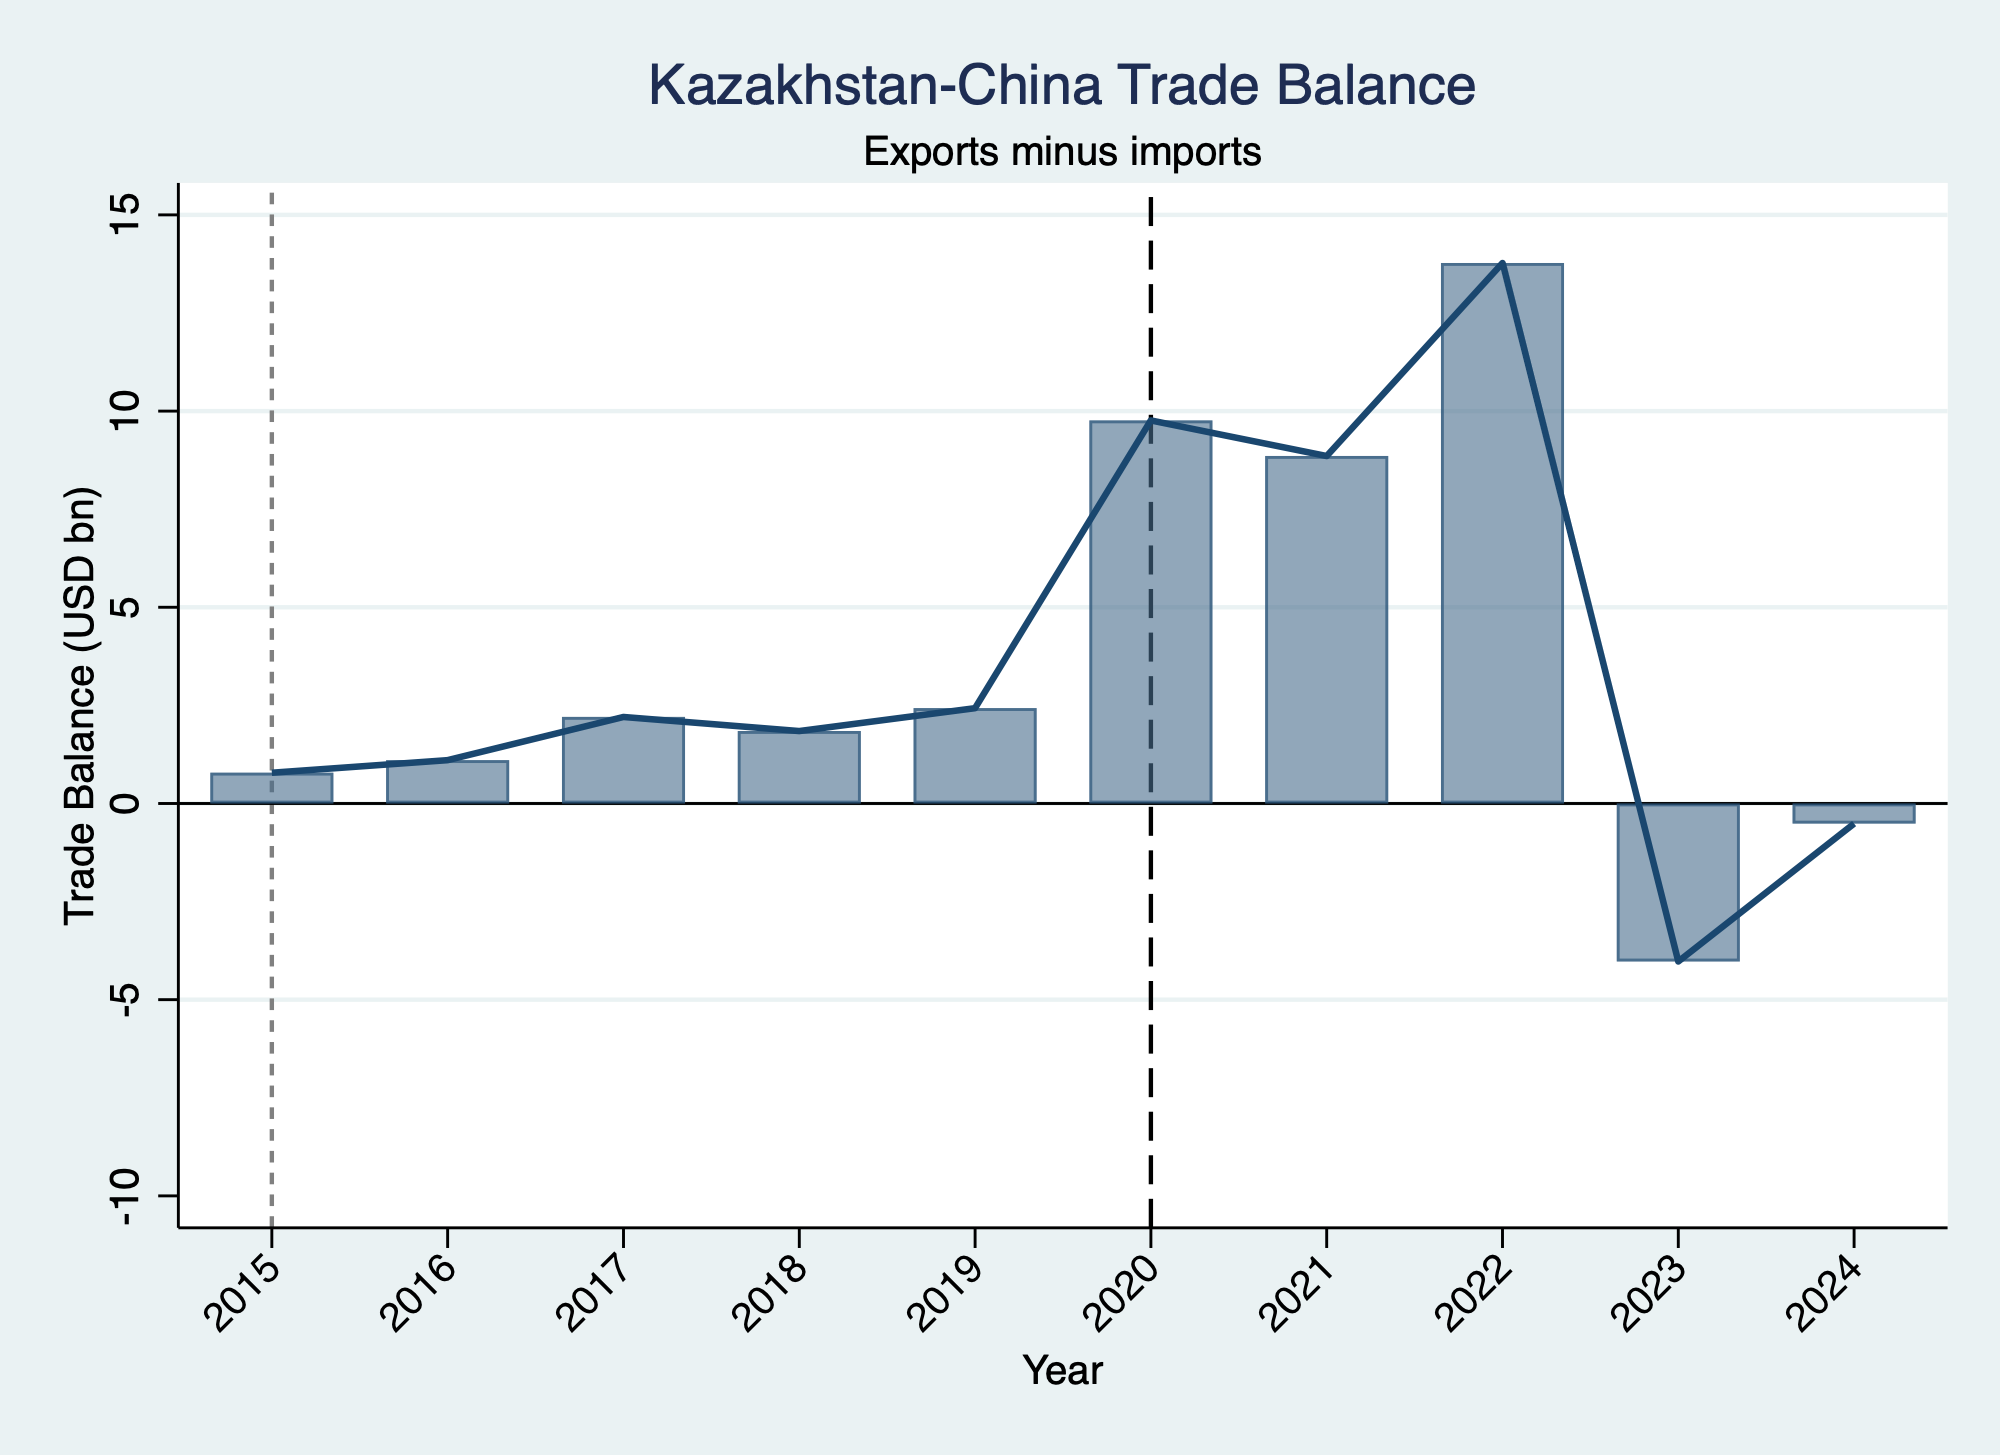
\includegraphics[width=0.95\textwidth]{../figures/fig13_trade_balance.png}
\caption{Kazakhstan--China bilateral trade balance, 2015--2024. Source: author's calculations from WITS data.}
\label{fig:trade-balance}
\end{figure}

As Figure~\ref{fig:trade-balance} shows, the deficit also highlights the limits of policy instruments aimed primarily at trade facilitation. Faster corridors, customs cooperation, and localization agreements can increase volumes, but they do not automatically create domestic technological capacity. Without industrial upgrading, improved connectivity may simply make the existing division of labor more efficient.

\subsection{Comparison with Russia and the European Union}

A comparison with Russia and the European Union reinforces the point that Kazakhstan's challenge is not reducible to one bilateral relationship. Kazakhstan's wider external trade remains diversified across several major partners, which weakens a narrow dependence claim. At the same time, the China relationship is especially important because it illustrates how diversification in partner count does not necessarily prevent peripheral specialization in trade composition.

Russia remains important because of geographic proximity, inherited Soviet-era industrial links, and Eurasian Economic Union rules. The European Union remains important as a market, investor, and regulatory reference point. Yet neither relationship eliminates the specific structural pattern visible in Kazakhstan--China trade. Multivectorism spreads Kazakhstan's external ties across partners, but the distribution of partners does not by itself determine the composition of production.

\section{Developmental Risk and Structural Constraints}

The developmental risk identified here is not immediate collapse or simple dependency, but the gradual entrenchment of a trade pattern that limits industrial upgrading. When exports remain concentrated in primary goods and imports remain concentrated in higher value-added manufactures, the domestic economy has fewer opportunities to develop the productive capabilities associated with sustained structural transformation. The risk is therefore cumulative: each additional round of commodity-led integration may deepen connectivity while leaving Kazakhstan's long-run development model unchanged.

Domestic political economy conditions help explain why the commodity pattern persists. Extractive sectors generate large export revenues and remain institutionally entrenched, while industrial upgrading requires coordinated policy, infrastructure, skills formation, and sustained support for manufacturing. As a result, even when official strategy documents emphasize diversification and localization, implementation often falls short of altering Kazakhstan's position in the bilateral value chain.

The automotive sector illustrates the ambiguity of localization. Chinese manufacturers can use Kazakhstan's Eurasian Economic Union (EAEU) membership and industrial zones to assemble vehicles for local and regional markets. Such projects may create jobs and support domestic manufacturing statistics, but assembly is not the same as deep industrial upgrading. If high-value components, design, technology, branding, and strategic control remain external, Kazakhstan's position in the value chain remains limited.

Public skepticism toward Chinese economic activity also constrains policy. Protests over land reform, opposition to large Chinese industrial projects, and public concern about Xinjiang have created a domestic environment in which the government must manage Chinese engagement carefully. These societal constraints do not reverse the structural trade pattern, but they make the political management of deeper integration more difficult.

\section{Strategic Responses for a Small-to-Middle Power}

The policy problem facing Kazakhstan is not whether to engage China, but how to engage China without allowing the relationship to reproduce a peripheral trade position. A small-to-middle power cannot usually compel a larger industrial economy to change the terms of exchange directly. It can, however, shape the conditions under which external capital, market access, logistics corridors, and technology enter the domestic economy. The relevant strategic question is therefore not exit, but bargaining: how can Kazakhstan use its geography, resource base, transit role, and multivector diplomacy to improve its position within regional value chains?

One useful theoretical lens is hedging. In the international relations literature, hedging refers to the attempt by smaller states to avoid full alignment with any single great power while extracting benefits from multiple relationships. Kazakhstan's multivectorism already resembles this logic. It maintains ties with China, Russia, the European Union, Turkey, the Gulf states, and international financial institutions, thereby reducing the diplomatic costs of overreliance on one partner. Yet hedging is not sufficient if it remains only diplomatic. A state can hedge externally while remaining structurally locked into commodity exports internally. For Kazakhstan, the task is to convert diplomatic hedging into productive hedging: using competition among large powers to secure investment terms that build domestic capabilities rather than simply expanding trade volume.

A second relevant concept is institutional balancing. Instead of balancing a large power militarily, small and middle states can use institutions, standards, and multilateral agreements to widen their bargaining space. Kazakhstan can do this by embedding China-related projects in wider regulatory and financing frameworks that include European, Turkish, Gulf, Japanese, Korean, and multilateral development-bank participation. Joint financing and shared standards make it harder for any single partner to dominate project design, procurement, or debt terms. They also allow Kazakhstan to compare offers across partners and attach stronger conditions to market access, including local procurement, workforce training, technology transfer, and environmental standards.

The most important strategic response is selective industrial policy. Kazakhstan should not try to diversify into every manufacturing sector at once. A more realistic strategy is to identify sectors connected to existing advantages but capable of moving beyond raw materials. These include metals processing, uranium-related services, petrochemicals, battery inputs, agricultural processing, logistics services, rail equipment maintenance, renewable-energy components, and selected automotive parts. The aim would be to move from exporting commodities to exporting processed inputs, intermediate goods, and services linked to those commodities. This is a more plausible upgrading path than attempting to leap immediately into advanced final-goods manufacturing.

To make this strategy credible, Kazakhstan would need to tie foreign investment approvals to measurable upgrading requirements. Localization should be defined not only by final assembly or Kazakhstani registration, but by domestic value added, supplier development, training, and technology absorption. Automotive assembly, for example, should count as industrial upgrading only if it generates local component suppliers, engineering capacity, after-sales service networks, and exportable production capabilities. Otherwise it risks becoming a statistical substitute for development rather than development itself. Investment incentives should therefore be conditional, time-limited, and reviewed against clear performance benchmarks.

Kazakhstan can also use its transit position more strategically. The Middle Corridor and China--Europe rail routes give Kazakhstan leverage, but transit fees alone will not transform the economy. Corridor strategy should be linked to logistics upgrading: warehousing, customs technology, cold-chain infrastructure, repair services, digital tracking, insurance, trade finance, and regional distribution hubs. These activities create more domestic value than simply allowing goods to pass through the country. If Kazakhstan becomes only a corridor, it earns rents. If it becomes a logistics and processing platform, it can build capabilities that support diversification.

Another practical strategy is standards diversification. China offers scale, speed, and infrastructure capacity, while the European Union offers regulatory standards, technology requirements, and access to high-value markets. Kazakhstan can use both, but for different purposes. Chinese demand and investment can support volume and infrastructure; European standards can discipline upgrading in carbon reporting, product quality, traceability, and industrial governance. Rather than treating China and the EU as substitutes, Kazakhstan can use EU-facing requirements to raise the quality of domestic production while using Chinese-linked corridors to expand market access. This is a form of multivectorism directed at industrial capability rather than diplomatic balance alone.

Regional coordination is also essential. Individually, Central Asian states often negotiate with China from positions of limited leverage. Collectively, they control critical transit geography, energy routes, water-sensitive agricultural zones, and a growing regional consumer market. Kazakhstan could work with Uzbekistan, Kyrgyzstan, Tajikistan, and Turkmenistan to harmonize selected customs procedures, infrastructure standards, and investment screening rules. Such coordination would not require anti-Chinese alignment. Its purpose would be to prevent a race to the bottom in which each state offers weaker conditions to attract the same external capital. Regional bargaining can strengthen small-state agency without requiring confrontation.

Finally, Kazakhstan needs domestic institutions capable of implementing this strategy. Industrial upgrading requires more than policy slogans. It needs technical agencies that can evaluate projects, monitor local-content claims, support supplier development, coordinate vocational education, and withdraw incentives from firms that do not meet performance targets. It also requires transparency, because opaque deals can deepen public suspicion of Chinese projects and weaken the legitimacy of diversification policy. Domestic trust is therefore part of external strategy. If citizens believe China-related projects mainly benefit elites or foreign firms, even economically useful projects will become politically fragile.

These strategies do not eliminate the core--periphery problem immediately. They do, however, identify ways a small-to-middle power can act within asymmetric conditions. Kazakhstan's leverage lies in combining several assets: geographic indispensability, commodity endowments, diplomatic flexibility, access to multiple external partners, and the ability to set domestic investment rules. The central challenge is to use those assets not merely to attract more trade, but to bargain for the capabilities that make future diversification possible.

\section{Conclusion}

This study has argued that Kazakhstan's economic relationship with China is better understood through world-systems theory than through the strongest versions of interdependence or dependence frameworks. The evidence does not require the claim that Kazakhstan and China have become deeply interdependent in a strict bilateral sense, since neither is the other's dominant trade partner across the entire system. The more persuasive finding is that their trade relationship remains structurally organized around a core--periphery exchange, in which Kazakhstan supplies raw materials and China supplies higher value-added manufactures.

This pattern does not automatically make Kazakhstan dependent in a narrow trade-share sense, but it does create a developmental risk by reinforcing commodity specialization and limiting industrial upgrading. The central policy challenge is therefore not simply to reduce trade with China, but to change the composition of Kazakhstan's production and exports so that participation in regional trade no longer reproduces peripheral status. Multivector diplomacy may broaden Kazakhstan's room for maneuver internationally, but without domestic industrial policy and export diversification it cannot by itself alter the country's structural position in the bilateral value chain.

The policy implication is direct. Kazakhstan's goal should not be disengagement from China, which would be costly and unrealistic. The more important goal is to use Chinese demand, transit investment, and regional connectivity in ways that expand domestic productive capacity. That requires export diversification, stronger industrial policy, better supplier development, deeper skills formation, and investment conditions that move beyond assembly toward technology transfer and higher local value added. In practical terms, Kazakhstan's multivectorism must become more developmental: a strategy for bargaining with large powers over capabilities, standards, technology, and value added, rather than only a strategy for preserving diplomatic balance.

\section*{Declaration of Competing Interest}

The authors declare that they have no known competing financial interests or personal relationships that could have appeared to influence the work reported in this paper.

\newpage
\section*{References}

\noindent Amineh, M. P., and Li, S. (2025). The structural challenges of transnationalizing the China-led BRI: The case of Pakistan. \textit{Journal of Contemporary Asia}. \url{https://doi.org/10.1177/0169796X251369694}

\noindent Balassa, B. (1965). Trade liberalisation and ``revealed'' comparative advantage. \textit{The Manchester School}, 33(2), 99--123.

\noindent Bitabarova, A. U. (2018). Unpacking Sino-Central Asian engagement: The case of Kazakhstan. \textit{Asian Security}, 14(1), 30--55.

\noindent Bitabarova, A. U. (2019). Kazakhstan's perspective on the Belt and Road Initiative. \textit{Asian Studies Review}, 43(4), 595--613.

\noindent Blackwill, R. D., and Harris, J. M. (2016). \textit{War by other means: Geoeconomics and statecraft}. Harvard University Press.

\noindent Brown, A. J. (1949). \textit{Applied economics: Aspects of the world economy in war and peace}. George Allen \& Unwin.

\noindent Cannon, B. J., and Rossiter, A. (2025). Rethinking and arresting Eurasian hegemony: The centrality of Central Asia to Indo-Pacific strategies. \textit{International Affairs}, 101(4), 1193--1212.

\noindent Caspian Policy Center. (2023). \textit{China--Kazakhstan bilateral relations}. \url{https://www.caspianpolicy.org}

\noindent Castellano, A., and Castillo, R. (2024). Chinese state capital as a partner for resource-based structural transformation? The Belt and Road Initiative and downstream linkages in Bolivia and Kazakhstan. \textit{The European Journal of Development Research}. \url{https://doi.org/10.1057/s41287-024-00640-1}

\noindent Chen, X., et al. (2025). The influence of the Belt and Road Initiative on China's advancement in global value chains and developing economies: A systematic review. \textit{The Chinese Economy}, 58(4), 87--114.

\noindent Clarke, M. (2015). Kazakhstan's multi-vector foreign policy: Diminishing returns in an era of great power ``pivots''? \textit{The Asan Forum}.

\noindent Contessi, N. P. (2015). Foreign and security policy diversification in Eurasia: Issue splitting, co-alignment, and relational power. \textit{Problems of Post-Communism}, 62(5), 299--311.

\noindent Georgia Foundation for Strategic and International Studies (GFSIS). (2025, March). \textit{Current trends in political and economic relations between China and Kazakhstan}. \url{https://gfsis.org}

\noindent Haji, A. A., and Khattak, S. H. (2025). Geopolitical chessboard: China's Belt and Road Initiative and shifting power dynamics. \textit{Discover Global Society}. \url{https://doi.org/10.1007/s44282-025-00200-w}

\noindent Goh, E. (2007). Great powers and hierarchical order in Southeast Asia: Analyzing regional security strategies. \textit{International Security}, 32(3), 113--157.

\noindent He, K. (2008). Institutional balancing and international relations theory: Economic interdependence and balance of power strategies in Southeast Asia. \textit{European Journal of International Relations}, 14(3), 489--518.

\noindent Hirschman, A. O. (1945). \textit{National power and the structure of foreign trade}. University of California Press.

\noindent Kassenova, N. (2017). China's Silk Road and Kazakhstan's bright path: Linking dreams of prosperity. \textit{Asia Policy}, 24(1), 110--116.

\noindent Keohane, R. O., and Nye, J. S. (1977). \textit{Power and interdependence: World politics in transition}. Little, Brown.

\noindent Kuik, C.-C. (2008). The essence of hedging: Malaysia and Singapore's response to a rising China. \textit{Contemporary Southeast Asia}, 30(2), 159--185.

\noindent Laruelle, M., and Peyrouse, S. (2012). \textit{The Chinese question in Central Asia: Domestic order, social change, and the Chinese factor}. Hurst \& Company.

\noindent Lim, G., Tjia, L. Y.-N., and Murashkin, N. (2025). Opportunities and challenges of China's economic ties with Kazakhstan: Looking back to look forward. \textit{The Chinese Economy}, 58(1). \url{https://doi.org/10.1080/10971475.2024.2373643}

\noindent Luttwak, E. N. (1990). From geopolitics to geo-economics: Logic of conflict, grammar of commerce. \textit{The National Interest}, 20, 17--23.

\noindent Mercator Institute for China Studies (MERICS). (2022). \textit{Kazakhstan's three-way balancing act between competing powers is under pressure}. \url{https://merics.org}

\noindent Neafie, W. (2022). Producing the Eurasian land bridge: A case study of geoeconomic contestation in Kazakhstan. \textit{Geopolitics}, 29(1), 1--28.

\noindent Pepe, J. M. (2021). \textit{The Middle Corridor as part of China's Belt and Road Initiative}. MERICS.

\noindent Peyrouse, S. (2012). Central Asia's evolving foreign policy: Multi-vectorism, Russia, China, and the West. \textit{PONARS Eurasia Policy Memo No. 230}.

\noindent Primiano, C. B., and Kudebayeva, A. (2025). A bumpy ride for China's Belt and Road Initiative in Kazakhstan: Findings from a university survey. \textit{Journal of Current Chinese Affairs}. \url{https://doi.org/10.1177/18681026231211354}

\noindent Rolland, N. (2017). \textit{China's Eurasian century? Political and strategic implications of the Belt and Road Initiative}. National Bureau of Asian Research.

\noindent Stronski, P., and Sokolsky, R. (2024, May). China, Russia, and power transition in Central Asia. \textit{Foreign Policy Research Institute}. \url{https://www.fpri.org}

\noindent Summers, T. (2016). China's ``New Silk Roads'': Sub-national regions and networks of global political economy. \textit{Third World Quarterly}, 37(9), 1628--1643.

\noindent Vanderhill, R., Lutsevych, O., and Buras, P. (2021). How Kazakhstan is navigating its relations with China. \textit{International Affairs}, 97(5), 1337--1354.

\noindent Wallerstein, I. (1974). \textit{The Modern World-System I: Capitalist Agriculture and the Origins of the European World-Economy in the Sixteenth Century}. Academic Press.

\noindent World Bank Group. (2020). \textit{The Belt and Road Initiative: Kazakhstan country case study}. World Bank.

\end{document}
